
% !TEX encoding = UTF-8 Unicode

%!TEX TS-program = xelatex
%!TEX encoding = UTF-8 Unicode

\documentclass[oneside,12pt]{book}
\usepackage[left=2cm,top=1cm,right=3cm,nofoot]{geometry}                % See geometry.pdf to learn the layout options. There are lots.
\geometry{a4paper}                   % ... or a4paper or a5paper or ...
\usepackage{tabularx}

\usepackage{xltxtra,xunicode}
\defaultfontfeatures{Mapping=tex-text}
\usepackage[french]{babel}
\usepackage{listings}
\usepackage{graphicx}
\usepackage[linktocpage]{hyperref}
\usepackage{hyperref}

\newcommand\don[5]{
\textbf{#1} \\
#2
\begin{itemize}
\item{ \textbf{jet}: #3}
\item{ \textbf{Cout}: #4}
\item{ \textbf{Page}: #5}
\end{itemize}
\vspace{0.5cm}
}


\title{Chicago : Scénario découverte}
\author{Renaud "ObiWan" Guezennec}
\date{}

%\let\origdescription\description
%\renewenvironment{description}{
%  \setlength{\leftmargini}{0em}
%  \origdescription
%  \setlength{\itemindent}{1em}
%}

\begin{document}

\maketitle \clearpage
\tableofcontents \clearpage

\chapter{Synopsis}
Des militaires fous aidés par un vampire ambitieux ont kidnappé une vampire illégale (Lizzy) et des SDF. \\
Les SDF servent de cobayes pour des expériences, ils reçoivent du sang de Lizzy. Le but est de créer des soldats plus résistant.\\
La disparition de SDF (garde manger de certains vampires) commence à se voir et des corps sont retrouvés totalement exsangues.\\
Le prince envoie son meilleur agent sur le coup: Victoria. \\
Victoria est la vampire qui a créée Lizzy en toute illégalité et elle ne sait pas que Lizzy est l'élément clé de ces recherches.\\ 
Le bras droit politique du prince prévient les militaires que Victoria est en approche.\\
Quand Victoria arrive pour les défoncer, elle est obligée de se rendre car ils menacent Lizzy. \\
Le lendemain soir, les joueurs débarquent pour régler ça. Retrouver Victoria et mettre fin à ces enlèvement de SDF.\\
Le centre d'opération des militaires est un hopital respectable en plein centre de Chicago.\\



\chapter{Les personnages}
\begin{flushleft}
\clearpage
\section{Ken Cliff}
\begin{description}
\item[Nom:]{Ken Cliff}
\item[Clan:]{Gangrel}
\item[Concept:]{Etudiant}
\item[Age:]{23 ans}
\item[Fiche de Perso:]{\url{http://nwod.rolisteam.org/fr/pdf/31}}
\item[Histoire]{
Tu es venu à Chicago pour essayer de convaincre ta copine de revenir. Elle travaille dans un bar, tu y es allée et la situation est partie en sucette. Tu t'es énervé, le videur et des client du bar aussi. Ils étaient neuf sur toi. Tu en as calmé six avant de te retrouver dehors. Devant ces prouesses, un mec t'a proposé une plus grande puissance. Elle ne vient pas sans coût mais elle te donnerais les moyens d'accomplir tous tes désirs. Tu as accepté, il t'a étreint. 
}
\end{description}


\vspace{0.5cm}
\subsection{Disciplines}
\vspace{0.5cm}
\don{Métamorphose: Aspect du prédateur}{La capacité la plus basique de cette discipline colle parfaitement aux Gangrels. Elle permet de projeter une impression surnaturelle de férocité sauvage. De plus, elle immunise le vampire aux réactions habituelles de peur lorsqu'il rencontre un vampire plus agé et puissant que lui. On considère que le gangrel est de la même Puissance de Sang que le vampire rencontré si celui ci lui est supérieur.}{Aucun}{Aucun}{138}
\don{Métamorphose: Refuge de terre}{Permet de fusionner avec la terre (pratique pour se cacher du soleil)}{Aucun}{1 vitae}{138}
\don{Métamorphose: Griffe de la bête}{Le vampire obtient des griffes surnaturelles}{Aucun}{1 vitae}{134 }


\clearpage

\section{Kurt Jackson}
\begin{description}
\item[Nom:]{Kurt Jackson}
\item[Clan:]{Mekhet}
\item[Concept:]{Ninja en devenir}
\item[Age:]{35 ans}
\item[Fiche de Perso:]{\url{http://nwod.rolisteam.org/fr/pdf/33}}
\item[Histoire]{
Tu travaillais pour la mafia de Chicago, tu étais un tueur chargé d'éliminer des personnes le plus discrètement possible. Un jour, tu as reçu l'ordre de tuer un gros poisson. La somme était tentante. Il est tombé dans ton piège mais cela ne lui a rien fait. En fait, il était ton client et ta cible. C'était un test. Tu as réussi à le trouver, et à l'attaquer. Il a fait de toi son nouveau chef de la sécurité, cela implique quelles modifications et principalement, de devenir vampire.
}
\end{description}

\vspace{0.5cm}
\subsection{Disciplines}
\vspace{0.5cm}
\don{Dissimulation: Masque de Tranquillité}{Le vampire ne peut-être identifier par un nouveau vampire. La souillure du prédateur est invisible. Il passe pour un humain pour les sens d'un autre vampire.}{Aucun}{Aucun}{134 }
\don{Dissimulation: Hypnotisme}{cache un petit objet sur le corps du vampire }{Astuce + larcin + Dissimulation [6dés]}{}{117}
\don{Dissimulation: Manteau de nuit}{le vampire devient invisible. Le pouvoir efface la présence du vampire dans l'esprit des gens. Il marche même à travers une caméra en direct. Sur des images enregistrées, il apparaît comme tout vampire. Il peut courir à travers une foule dans cette forme là, les gens s'écartent. Une personne peut de façon inconsciente laisser ouverte une porte plus longtemps derrière elle pour le laisser passer. Le pouvoir s'arrête si le vampire touche un objet autre que le sol: poignée, coup de poing, coup de poignard… }{Intelligence + furtivité + Dissimulation [7dés]}{}{118}



\clearpage
\section{Alice}
\begin{description}
\item[Nom:]{Alice}
\item[Clan:]{Mehket}
\item[Concept:]{Enquêteuse de l'ombre}
\item[Age:]{22 ans}
\item[Fiche de Perso:]{\url{http://nwod.rolisteam.org/fr/pdf/30}}
\item[Histoire]{ 
Jeune fille, très savante et sérieuse. Tu travaillais dans une librairie. Tard le soir, un homme te rendait visite. Il est tombé en admiration devant ton savoir. Tu pensais qu'il voulait t'offrir du travail plus valorisant qu'une librairie de quartier. En quelques sortes, il l'a fait. Il t'a étreint. Tu devenue une vampire. Tu as l'éternité pour satisfaire ta curiosité maintenant.
}
\end{description}

\vspace{0.5cm}
\subsection{Disciplines}
\vspace{0.5cm}
\don{Auspex: Sens accrue}{Tous les sens sont améliorés }{Aucun}{Aucun}{118}
\don{Auspex: Lecture des auras}{lire les auras: connaître les sentiments du sujet: colère, mensonge , amour ..., permet de connaître sa nature: humain, vampire…}{Astuce + empathie + Auspex[9dés]}{}{118}
\don{Auspex: Toucher de l'esprit}{Connaître le passé d'un objet. De telles impressions peuvent apprendre au vampire qui a tenu l'objet en dernier, quand cela s'est produit, et même à quoi il a servi en dernier.}{Astuce + Occulte + Auspex[9dés]}{Aucun}{118}

\clearpage
\section{Eugène W. Helligton}
\begin{description}
\item[Nom:]{Eugène W. Helligton}
\item[Clan:]{Ventrue}
\item[Concept:]{Chef autoritaire}
\item[Age:]{48 ans}
\item[Fiche de Perso:]{\url{http://nwod.rolisteam.org/fr/pdf/34}}
\item[Histoire]{
Tu étais dans une soirée de gala pour une association et tu as sympathisé avec une jeune femme. Elle semblait amusée par tes tentatives. Un serveur a renversé du champagne sur la demoiselle, tu as copieusement insulté le pauvre homme et exiger son renvoi. Devant cette démonstration d'autorité, tu as clairement marqué des points. Pour te remercier, elle t'a fait vampire.
}
\end{description}

\vspace{0.5cm}
\subsection{Disciplines}
\vspace{0.5cm}
\don{Domination: Ordre}{Donner un ordre simple}{Intelligence + Intimidation + Domination [9dés] (Opposé à résolution + puissance du sang de la cible)}{Aucun}{130}
\don{Domination: Hypnotisme}{Implante un faux souvenir ou une fausse pensée.}{Intelligence  + expression + domination [8dés] ( opposé à Résolution + puissance du sang de la cible)}{Aucun}{130}
\don{Domination: Esprit distrait}{Permet de fouiller dans les pensées, pour fouiller ou remodeler. Peut troubler l'équilibre mental de la cible.}{Astuce + Persuasion + Domination [8dés] - résolution de la cible}{}{131}



\clearpage
\section{Emily Watts}
\begin{description}
\item[Nom:]{Emily}
\item[Clan:]{Daeva}
\item[Concept:]{Papillon de nuit}
\item[Age:]{18 ans}
\item[Fiche de Perso:]{\url{http://nwod.rolisteam.org/fr/pdf/32}}
\item[Histoire]{
Tu as toujours aimé avoir plein d'hommes autour de toi. Tu es une très jolie jeune fille et tu le sais. Tu utilisais ton charme pour séduire des hommes et te faire offrir des choses. Ainsi tu as pu rentré dans les plus grandes boîtes de Chicago. Une femme identifia ton petit jeu, elle t'a dit qu'elle faisait comme toi dans sa jeunesse (elle semblait plus jeune que toi). Finalement, vous avez sympathisé et elle t'a proposé la meilleure drogue que tu as jamais testé. Tu as accepté et est devenue une vampire.
}
\end{description}
 

\vspace{0.5cm}
\subsection{Disciplines}
\vspace{0.5cm}
\vspace{0.5cm}
\don{Majesté: Révérence}{Captiver un public, attirer l' attention}{Présence + Expression + Majesté [9dés]}{}{134}
\don{Majesté: Révélation}{La victime sera d'humeur à partager tous ses secrets.}{Manipulation + Persuasion + Majesté [7dés] ( opposé au Calme + puissance du sang de la cible) }{}{135}
\don{Majesté: Transe}{La victime admire et aime le vampire}{Manipulation + Empathie + Majesté[9dés]}{}{136 }




\chapter{Introduction à Vampire Le Requiem}
\section{Le système}

Le jeu utilise des dés à 10 faces. \\
Les jets sont souvent un attribut plus une compétence. Le joueur compte les points noirs sur sa fiche. Cela lui donne le nombre de dés qu'il doit lancer. Un dés qui affiche 8, 9 ou 10 (souvent représenté par un 0) est une réussite. Le 10 permet de relancer encore. \\
Exemple: Je demande à Kurt de faire un jet pour être discret:\\ Dextérité + Furtivité => 6dés.\\
\vspace{0.5cm}
Le résultat des dés est : 10, 9, 3, 1, 8, 4. Kurt a déjà obtenu 3 succès. Il relance le 10, le dés refait encore 10. C'est un 4ème succès pour Kurt. Il relance, le dés fait 2. C'est terminé, score final 4 succès. \\
Les gardes devront faire 4 succès (ou plus) pour trouver Kurt (en cas d'égalité, c'est le défenseur qui gagne. Dans notre cas, Kurt «attaque» en tentant de s'inflitrer discrètement).
\\
\subsection{Bonus aux jets}
Les jets physiques peuvent être augmenter par la dépense d'un point de sang (Vitae) (pour un bonus de 2 dés).\\
\vspace{0.5cm}
Exemple: Les personnages doivent fuir en vitesse par les toits. Pour sauter sur le toit voisin, il faut faire 3 succès.\\ Emily n'est pas une athlète, elle dépense 1 point de sang (vitae) pour avoir un bonus.
\\
Les points de volonté offre un bonus de 3 dés pour n'importe quel jet. \\
Récupérer des points de sang se fait en se buvant le sang d'une personne ou d'un animal.\\
Un humain entier redonne 10 points de sang.
Prendre plus de 4 points sur la même personne peut le tuer s'il n'est pas soigné très vite; 10 point le tue.\\

\subsection{Initiative}
L'initiative : chaque joueur lance un dés 10, et ajoute la valeur de dés à son score d'initiative de sa fiche.\\
La plus forte initiative commence.\\
\vspace{0.5cm}

\subsection{Combat}
Pour les combats, il y a 4 types d'attaques:\\
-\textbf{Mains nues} : Force + Bagarre - la défense de l'adversaire.\\
-\textbf{Armes blanches} : Force + Arme blanches + Bonus de l'arme (2 un couteau, 3 une épée…) - défense de l'adversaire\\
-\textbf{Armes à feu}: Agilité + Arme à feu + Bonus de l'arme (2 pour un revolver, 3 un fusil automatique …)\\
-\textbf{Lancer d'arme} : Force + Athlétisme + Bonus de l'arme (2 un couteau) - défense de l'adversaire\\
\vspace{0.5cm}

Pas de défense sur les armes à feu. Le score de défense d'un adversaire diminue de 1 pour chaque attaque qu'il subit dans le tour. Au début du tour, les scores de défense sont ré-initialisés.\\
\vspace{0.5cm}
\subsection{Dégâts}
Les dégâts subit sont le nombre de succès de l'attaquant. Il existe 3 types de dégâts: Contondants, létaux, et aggravés.\\
\vspace{0.5cm}

Contondants: coup de poing, batte de baseball… (ce qui fait des bosses)\\
Létaux: Arme à feu, couteau (ce qui fait des trous)\\
Aggravés: le feu (sur les vampires), et les griffes de \textbf{Ken Cliff}\\

\subsection{Santé}
\vspace{0.5cm}
Un vampire avec 7 point de santé: il lui faudra 21 dégâts contondants pour mourir ou 14 létaux ou 7 aggravés.\\
Dans la barre de santé, les contondants sont représentés par une barre verticale: | \\
Les dégâts létaux sont réprésentés par des +, les aggravés par des *. \\


\section{C'est quoi un vampire?}
Un vampire est un humain dont le corps est mort. Le cœur ne bat plus, le sang ne circule plus.\\ 
Cependant pour activer son corps, le vampire est obligé de dépenser un point de sang (vitae) le soir au réveil. Ainsi, il peut bouger normalement jusqu'au lever du soleil.\\ 
Manger, boire, fumer, digérer demande la dépense d'un autre point de sang (vitae) permettant de réactiver ses fonctions pour quelques minutes/heures. Cela peut aussi marcher pour se soigner, les plaies se referment.\\ 
\vspace{0.5cm}
Le vampire craint le soleil et le feu.\\  
En échange de ces sacrifices, il a gagné une résistance à la douleur et des pouvoirs appelés Discipline.
Il existe cinq grand clans de vampire:\\ 

\vspace{0.5cm}
\begin{tabularx}{\linewidth}{|c|c|c|X|}
\hline 
Clan & Stéréotype & Discipline de clan & Défaut \\ 
\hline 
Ventrue & Chef autoritaire, fou, noble, gourmand & Domination & Devient fou \\ 
\hline 
Mehket & Ninja/assassin ou enquêteur occulte & Auspex & Craint plus le feu que les autres \\ 
\hline 
Gangrel & Les bêtes & Métamorphose & Les jets mentaux sont plus durs. \\ 
\hline 
Deava & Succube, artiste & Majesté & Du mal à contrôler leurs envies \\ 
\hline 
Nosfératu & Moche et collectionneur & Cauchemar & Les jets sociaux sont plus difficiles. \\ 
\hline 
\end{tabularx} 
\vspace{0.5cm}

Il existe des disciplines accessible par tout vampire.
Les vampires ont en eux la Souillure du Prédateur. Sorte d'instinct animal qui peut forcer un vampire dans certain cas.\\ 
\vspace{0.5cm}
La souillure du prédateur réagit face à la souillure d'un autre prédateur, lors de leur première rencontre. Cela permet à un vampire d'identifier un vampire inconnu. 
Les personnages doivent faire un test de résolution + calme.\\ 
\vspace{0.5cm}
Si les deux réussissent, il ne se passe rien. Ils savent cependant qu'il y a un vampire nouveau à proximité, ils ont la direction. \\ 
\vspace{0.5cm}
Si un échoue, le prédateur prend le pas. Si l'autre vampire a une plus grande puissance du sang, le prédateur 
voudra fuir face au prédateur d'en face. S'ils sont de puissance égale, le perdant montre les crocs, en mode intimidation. Dans le cas, ou l'adversaire a une puissance de sang inférieure, le prédateur lance la chasse.\\ 
\vspace{0.5cm}
Les pouvoirs de Kurt et Cliff ont un impact à ce niveau. 
Kurt fait le jet mais son adversaire, non. \\
Cliff fait le jet mais s'il rare, il ne fuit pas, il passe en mode intimidation. Si son adversaire rate, il passe aussi en mode intimidation ou fuite.


\section{Organisation du monde Vampirique}
Les vampires sont organisés en société monarchique. 
Un prince est le chef suprême des vampires dans la ville. C'est lui qui donne les territoires de chasse. \\
Il autorise la création de goules ou d'infants. Il a pour charge de garantir la sécurité des vampires et punit les vampires désobéissants. Le respect de la mascarade est primordial. Les humains ne doivent pas savoir. \\
Un prince peut lancer une chasse au sang sur un vampire hors la loi.
Il est interdit de boire un vampire jusqu'à sa mort (le diabler).


\section{Alimentation du vampire}
Facile, il boit du sang. Les jeunes peuvent boire du sang d'animaux mais il est bien moins bon que celui d'humain. \\
Les crocs sortent à volonté. Il suffit de lécher la plaie pour faire disparaître les traces de morsure. 


\chapter{Scénario}

Durée: 2h \\
États des relations en début de scénario:\\
\begin{center}
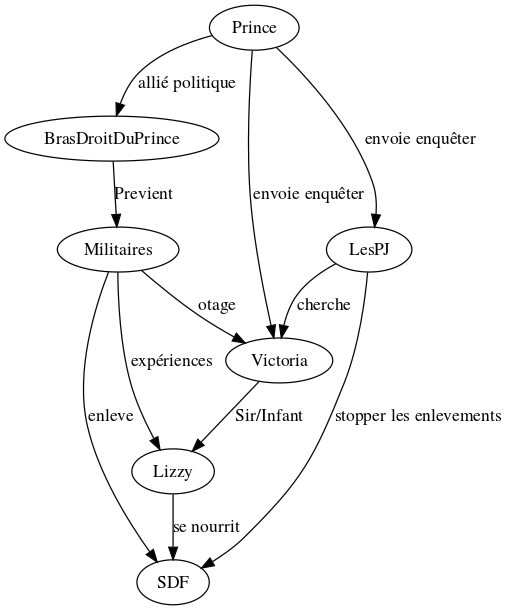
\includegraphics[width=0.6\linewidth]{scenario.png}
\end{center}


\section{Introduction}
Le Prince de la ville de Chicago a demandé aux PJ d'enqueter sur la disparition de Victoria.  \\
Victoria est la meilleure agent du prince. Elle est du clan Mehket et l'élément parfait pour réussir une enquête et neutraliser le problème. \\
Victoria a été envoyée sur une enquête de disparitions de SDF dans la ville.
Le prince pense que des vampires sont impliqués car les SDF sont retrouvés vidés de leur sang et morts. \\
Elle a contacté le prince (hier vers 3h du mat) pour dire que le problème a pour origine le Cook County Hospital. On sait que Victoria est rentré dans l'hopital mais n'est jamais resortie.
Le scénario démarre devant l'hopital. \\
\vspace{0.5cm}
En clair, la mission des PJ est d'enquêter et régler le problème des morts des SDF et en bonus de retrouver Victoria. \\
Après la disparition de Victoria, le prince n'a pas envie d'envoyer un autre bon élément. Il préfère envoyer plusieurs vampires sacrifiables.\\
Vous pouvez introduire le scénario en mode hors RP, pour démarrer devant l'hopital. Il est également possible de jouer la scène ou le prince leur demande (ordonne) d'aller mener l'enquête.
Démarrer la scène, par un tour de table de description physique des personnages (taille, style vestimentaire, couleur de cheveux, etc).

\section{Rentrer dans l'hopital}
Le but de cette scene est de proposer une scene de RP. Les personnages entrent dans une salle d'attente.\\ 
Quelques patients attendent.\\
Il y a une personne derrière une vitre qui donne les dossier à remplir (Pensez aux guichets de métro). \\
Une fois le dossier rempli, il est mis à disposition des docteurs. Quand un docteur est disponible, il prend un dossier et va chercher le patient dans la salle d'attente. Il y a un sas à franchir. \\
\vspace{0.5cm}
Plusieurs possibilité pour passer le sas:\\
\begin{itemize}
\item Se faire passer pour un malade (attention le corps d'un vampire est mort).\\
\item trouver une entrée de service pour s'infiltrer.\\
\item Laisser libre cours à l'imagination de vos joueurs.\\
\item Utilisation de pouvoirs sur la dame de l'accueil : Emily ou Eugène.
\end{itemize}

\vspace{0.5cm}
Laisser les réfléchir un temps. Quand ils sont dans la salle d'attente en train de se demander comment agir, un vigile reçoit un appel à la radio. Il y a visiblement un problème avec la caméra de surveillance de la salle. En effet, les vampires paressent toujours flou quand ils sont filmés ou photographier. \\
Il est également possible de voir un plan des étages de l'hopital. Il y une morgue au -1, le QG sécurité est au 8ème étage. Le bureau du directeur au 9eme, Le -2 et -3 sont des parkings. \\
\vspace{0.5cm}

\section{Les couloirs}
Si vos joueurs décident de se balader dans l'hopital, il faut faire jouer deux éléments:
-Les vigiles vont pouvoir les suivre grâce au caméra et ils ne vont pas laisser des inconnus visiter les locaux tranquillement.\\
-A part, les urgences les autres services sont généralement vides.\\
\vspace{0.5cm}
A vous d'ajouter un peu de tension, est-ce qu'il prennent l'ascenseur ou les escaliers ? etc…\\
S'ils visitent des zones non-décrites dans le scénario, il trouve une zone normale. Une morgue normale et vide, une maternité normale avec des bébés et des mamans qui dorment…

\section{Le QG sécurité}
Le premier objectif des joueurs est de se rendre aux QG sécurité. Ils y trouveront le chef de la sécurité. Un homme petit, du bide avec des taches de gras sur son polo bleu de sécurité. S'ils sont montés par l'ascenseur, il les attendra avec un fusil (en mode tranquille mais quand même). Il discutera d'abord, s'il se sent menacé il pointera son arme sur eux. \\ S'ils ont pris l'escalier, le chef de la sécurité envoie deux vigiles (en pleine forme) les intercepter et les mettre dehors.\\


\vspace{0.5cm}
Dans le QG, les caméras peuvent apprendre deux choses aux joueurs.\\
-Il y plein de trous dans les enregistrements d'hier. [note MJ: En effet, Victoria a effacé une partie des ses traces sauf la dernière].\\
-Sur le dernier enregistrement de Victoria, il est possible de la voir monter dans l'ascenseur au niveau 9. Elle passe une sorte de badge sur un mur de l'ascenseur. Il descendre tout en bas. Arrivé au niveau -3, l'image disparaît (toute noire) pour revenir 2 mins plus tard avec un ascenseur vide. \\


\vspace{0.5cm}
Le vigile est capable d'expliquer que le niveau -4 est confidentiel. Même lui ne peut pas y aller. Il sait que le directeur de l'hôpital conserve une clé dans son bureau.\\
Jet possible: 

\begin{itemize}
\item Astuce + Informatique pour rechercher dans les enregistrements 
\item Manipulation + Persuasion pour convaincre le vigile de lâcher les infos.
\item Manipulation + Intimidation pour convaincre le vigile de lâcher les infos.
\item Présence + Persuasion pour séduire le vigile et le convaincre de lâcher les infos (en échange de plaisirs sexuels).
\item Utilisation de pouvoirs : Emily ou Eugène.
\end{itemize}

\section{Bureau du directeur}
Le bureau est en réalité tout le 9ème étage (qui n'ait pas aussi grand que les autres étages). Il y a 2 pièces.\\
Le bureau de sa secrétaire et une grande porte donne sur le vrai bureau du directeur. \\
Bien sur, le bureau est vide, il est tard dans la nuit.\\
\vspace{0.5cm}
Pour franchir la grande porte, le vigile du QG a une clé, sinon:\\
\begin{itemize}
\item Astuce + Larcin (en discrétion)
\item Force + Athlétisme (en force)
\end{itemize}

Dans le bureau du directeur, les joueurs trouvent des meubles en acajou massif, des lampes designs, de vieux ouvrages … bref, il y a de l'argent dans ce bureau.\\
Un petit jet d'Astuce + investigation. Permet de trouver un coffre fort (derrière un tableau ou ailleurs). \\

\vspace{0.5cm}
Ouvrir le coffre fort: \\
\begin{itemize}
\item Astuce + Larcin, il faut faire au moins 4 ou 5 succès.
\item Utilisation du pouvoir «Toucher de l'esprit» d'Alice pour trouver la combinaison du coffre. Pensez à décrire un peu ce qu'elle voit. Une personne ouvre le coffre pour mettre le badge dedans…
\end{itemize}
\vspace{0.5cm}
Dans le coffre, ils vont trouver le badge et des lettres. Les lettres sont des courriers envoyés par le directeur d'un groupe de recherche: Lambda financé par l'US Marine et la CIA. Il remercie le directeur de sa discrétion pour les petites recherches réalisés par l'armée dans les sous-sols de son hôpital. Il y a aussi les factures pour le bureau en acajou, payer par l'armée bien sûr.

\section{Dans l'ascenseur}
S'ils y vont en mode tranquille. Leur rappeler que la meilleure agent du prince y a peut-être laisser la vie. \\
Si les joueurs n'y pensent pas, rappeler leur qu'il est possible d'utiliser le pouvoir: «Toucher de l'esprit» d'Alice sur le lecteur de carte de l'ascenseur.\\
Alice verra Victoria (pas flou, cette fois) passé le badge dans le lecteur, l'ascenceur descend. Passez le niveau -3, elle active son invisibilité (mais reste visible pour le pouvoir d'Alice) et prépare ses armes (couteaux).\\
Quand les portes s'ouvrent, une grande lumière blanche rentre. Alice ne voit pas ce que Victoria voit. \\
Victoria semble surprise de ce qu'elle voit. Elle coupe son invisibilité, et lache ses armes. Elle sort de l'ascenseur et le pouvoir d'Alice s'arrête.\\

\section{Au Quatrième sous-sol}
Quand les portes s'ouvrent, les joueurs sont accueillit par 2 soldats qui tirent pour tuer.
Ils ont 7 points de vie, 4 en défense et lance 10 dés pour leur attaque. Il font des dégâts létaux. Penser à jouer l'initiative. \\
Kurt et Cliff devrait régler cela en 2 tours. Kurt fait deux attaques par tour (sur le même type) et fait des dégâts létaux; Cliff lui fait des dégâts aggravés avec ses griffes mais n'attaque qu'une fois par tour.\\


\vspace{0.5cm}
Sinon, pour les personnage non combattant, il est possible de voir un grand couloir blanc. Il y a des traces de sang séché par terre (un peu). Au fond, une grande baie vitrée opaque forme un mur en arc de cercle. Deux scientifiques ouvrent la baie vitrée.\\


\vspace{0.5cm}
Tout l'intérêt de la scène est de savoir, s'il vaut mieux courir pour rentrer dans la pièce derrière la vitre ou combattre les 2 militaires.\\


\vspace{0.5cm}
Si des personnages partent immédiatement, ils n'ont pas besoin de faire de jet pour arriver à temps.\\
Ceux qui ont participer aux combats ou qui ont attendu qu'un adversaire soit hors combat devront faire les jets de dés.\\


\vspace{0.5cm}
La course poursuite est un peu technique mais cela apporte pas mal de tension à la table.\\
Les joueurs lancent :\\
Force + athlétisme\\


\vspace{0.5cm}
Le nombre de succès s'ajoute à la vitesse du personnage. Kurt a une vitesse de base de 12, il fait son jet d'athlétisme + Force et obtient 3 succès. Sa vitesse pour ce tour ci est de 15.\\ 
Pour info:\\ 
\begin{tabular}{|c|c|c|}
\hline 
Personnage & Vitesse & Jet d'athlétisme \\ 
\hline 
Kurt & 12 & 5dés \\ 
\hline 
Ken Cliff & 10 & 5dés \\ 
\hline 
Eugène & 9 & 4dés \\ 
\hline 
Alice & 9 & 4dés \\ 
\hline 
Emily & 10 & 5dés \\ 
\hline 
\end{tabular} 
\\
\vspace{0.5cm}
Pour la difficulté, je prends pour références 25 [ne pas dire la difficulté aux joueurs]. Si les joueurs prennent leur temps, et commence à courir quand la porte se referme derrière les scientifiques, Ils n'ont que deux tours pour faire le trajet (soit 15 de moyenne à leur jet).\\
Kurt n'aura pas de problème mais les autres cela peut-être plus dur. Si un personnage passe, il peut ouvrir la baie vitrée pour laisser passer les autres et faire tomber un peu la pression/tension.\\
\vspace{0.5cm}
Pour info, dans le couloir, il y a des cellules où sont enfermés des SDF kidnappé.\\

\section{Dans la bulle}
Au centre, une cage en verre de forme cylindrique. Dedans, une petite fille d'environ 8 ans.
Elle est une vampire (Faire les jets de Résistance à la souillure) et elle se traîne (Elle ne peut pas marcher). Elle a dans la main droite un bras humain dans la main gauche un ours en peluche dont les poils sont collés par le sang séché.\\
\vspace{0.5cm}
Au fond de la pièce, il y a Victoria attachée au mur (enchaînée). Les 2 scientifiques sont effrayés, ils essaient d'appeler du renfort, mais son mort de peur face aux joueurs. Ils connaissent leur vrai nature.
\vspace{0.5cm}
Les choses à faire, ici:
-Il faut nettoyer la zone donc tout détruire. Les joueurs n'ont pas forcément l'équipement, ni la connaissance pour le faire. Ils peuvent tuer les scientifiques.
-Il peuvent libérer Victoria. Elle est inconsciente, il lui faudra du sang. Soit du sang de vampire, soit d'un scientifique. Dans le cas, d'un scientifique elle le boira entier.
-L'objectif de Victoria, c'est de garder Lizzy la jeune vampire.
Un jet en intelligence + occulte ou politique peut donner l'information que cette Lizzy est illégale, le prince ordonnera une chasse au sang sur Lizzy et la personne qui l'a étreinte.\\
-Si les joueurs posent la question, elle explique que Lizzy est sa petite-petite-petite-petite-petite-fille (biologique). 
Elle et ses parents ont eu un accident de voiture. Le seul moyen de la sauver a été de la transformer en vampire. Elle a réussi a planquer Lizzy du Prince car il a confiance en elle. \\
\vspace{0.5cm}
Seulement, les militaires ont kidnappé Lizzy, il y a quelques mois. Elle a été trahi par un vampire. \\
\vspace{0.5cm}
Elle a cherché un temps, puis par hasard, c'est la mission du prince qui lui a permit de retrouver sa descendance.\\
\vspace{0.5cm}
-Victoria va alors demander aux joueurs leur intention [Laisser les répondre].\\
-Elle leur proposera de participer à son coup d'Etat. En devenant Prince de la ville, elle pourra autorisé Lizzy a vivre et elle sera remercier les joueurs pour leur aide. Pour les convaincre, elle jouera la carte émotion avec Alice et Kurt qui sont du même clan qu'elle.
-Si les joueurs se montrent agressifs envers elle, elle essaiera du fuir avec Lizzy. Elle n'est pas en mesure de combattre 5 vampires. D'ici quelques semaines sans problème.
-Victoria se propose de tout faire péter à l'étage (ellipse pas besoin de le jouer).

\section{Chez le prince}
Le lendemain soir, rendez-vous chez le prince.\\
Les joueurs doivent rapporter au prince les informations qu'ils ont obtenu.\\
\vspace{0.5cm}
Dans le cas, ou ils accusent Victoria d'avoir commit un acte illégal, le prince sera très en colère et accusera les joueurs de mensonges. Il ne peut croire que son meilleur agent ait commit cela.\\
Dans le cas où ils ont accepté le plan de Victoria, elle sera présente chez le prince. Elle passera à l'attaque et tuera le prince. Il y aura une petite purge dans l'élyséum pour supprimer les soutiens de l'ancien prince.\\

\section{Le prince est mort! Vive le nouveau Prince}
Une fois les actions martiales terminées, Victoria prendra place sur le trône de la ville. 
Elle fera un petit discours bidon, du genre que le Prince a laissé des militaires s'installer dans la ville pour faire des expériences. Il était faible etc…
Elle ne parlera pas de Lizzy. Pour finir, elle se tournera vers les joueurs. \\
Pour les remercier de lui avoir sauvé sa non-vie. Elle leur laisse 24 heures pour quitter la ville.\\
Elle ne veut pas de traite à proximité d'elle. S'ils reviennent en ville, ils seront tués.
Pour information, ils sont les seuls à connaître la vérité sur Lizzy. Ils ont de la chance de rester entier.\\


\end{flushleft}
\end{document}


